\documentclass[12pt]{article}
\usepackage[utf8]{inputenc}
\usepackage{graphicx} % Allows you to insert figures
\usepackage{amsmath} % Allows you to do equations
\usepackage{fancyhdr} % Formats the header
\usepackage{geometry} % Formats the paper size, orientation, and margins
\usepackage[style=authoryear-ibid,backend=biber]{biblatex} % Allows you to do citations - does Harvard style and compatible with Zotero
\addbibresource{Example.bib} % Tells LaTeX where the citations are coming from. This is imported from Zotero
\usepackage[english]{babel}
\usepackage{csquotes}
\renewcommand*{\nameyeardelim}{\addcomma\space} % Adds comma in in-text citations
\linespread{1.25} % About 1.5 spacing in Word
\setlength{\parindent}{0pt} % No paragraph indents
\setlength{\parskip}{1em} % Paragraphs separated by one line
\renewcommand{\headrulewidth}{0pt} % Removes line in header
\geometry{legalpaper, portrait, margin=1in}
\setlength{\headheight}{14.49998pt}

\begin{document}
\begin{titlepage}
   \begin{center}
        \vspace*{5cm}

        \Huge{Honors Thesis Title}

        \vspace{0.5cm}
        \LARGE{optional subtitle below}
            
        \vspace{3 cm}
        \Large{Gina Chun}
       
        \vspace{0.25cm}
        \large{Member Name 1, Member Name 2, Member Name 3, Member Name 4}
       
        \vspace{3 cm}
        \Large{Month Day, Year}
        
        \vspace{0.25 cm}
        \Large{Course Code}
       

       \vfill
    \end{center}
\end{titlepage}

\setcounter{page}{2}
\pagestyle{fancy}
\fancyhf{}
\rhead{\thepage}
\lhead{Group Name; Title of Document}

\section*{Outline}
\begin{enumerate}
   \item abstract
   \item intro, background, motivation
   \item dataset, model, three kinds of invariance
   \item method
   \item results, discussion, conclusion
   \item references/bibliography
\end{enumerate}

\section*{Motivation/Sales Pitch}
\subsection*{why carbon is important}

Carbon is one of the most important and widely investigated elements. Carbon is all around us in a variety of forms and is an area of study which has huge significance across many scientific fields and applications. Carbon is in living organisms and is essential for living organisms, thus the study of carbon would further develop the complex workings of the environment, ecosystems and the carbon cycle. It would also help the understanding of fossil fuels, aid the challenges of energy-related issues, and work towards solutions for climate change. Carbon materials are also intertwined in modern economic industries such as in steel, clothing, pigment, plastic and synthetic materials, and in electrodes and other similar electricity conducting machinery. Studying carbon allows for further advancement in these important industries which would lead to better and more easily accessible devices, tools, and products for general society.

\subsection*{why use machine learning}
As carbon is an important element, its versatility makes it a very complex subject of study. Carbon manifests in various physical forms, called allotropes, each with very different properties. Because of this, studying carbon can be difficult with conventional methods. Using Gaussian Approximation Potentials (GAP), machine learning can be much more cost and time efficient than traditional scientific methods of experimentation. Machine learning also opens up a new space of empirical methods for experiments that scientists cannot physically replicate with traditional techniques. For example, machine learning can be used for experiments in very small spatial scales or for large scale simulations all while maintaining high performance accuracy.

https://aip.scitation.org/doi/full/10.1063/5.0005084
\\ https://aip.scitation.org/doi/full/10.1063/5.0052870


\section*{Major Heading}
\subsection*{Subheading}

Lorem ipsum dolor sit amet, consectetur adipiscing elit. Sed blandit tortor ut pharetra auctor. Curabitur posuere massa vitae commodo malesuada. Lorem ipsum dolor sit amet, consectetur adipiscing elit. Ut aliquet lacus nec quam auctor, eget suscipit turpis efficitur. Sed convallis sed enim eu sagittis. Nunc pretium id lacus ut lacinia. Praesent gravida varius faucibus. Maecenas commodo pretium dignissim \autocite{cohen_quantifying_2020}. 

Etiam nec malesuada ex. Vestibulum laoreet purus nec metus egestas, sit amet fringilla ipsum laoreet. Pellentesque ornare, neque in convallis maximus, quam mi facilisis felis, sed cursus dui lectus sit amet felis. Proin finibus quis urna ut sollicitudin. Vestibulum congue, ex vitae suscipit efficitur, elit quam ullamcorper est, eget tempus mi velit eget mi. Integer eget nunc eu eros cursus bibendum. Vestibulum ultrices ligula quis nulla porta malesuada. Morbi vel mi vel erat tempor consectetur sed a arcu. Phasellus convallis nibh ut erat posuere, a pharetra ipsum viverra. Praesent scelerisque maximus urna. Nam mattis ac massa in scelerisque. Praesent vulputate feugiat diam id eleifend. Phasellus iaculis ut lectus vestibulum volutpat.

\begin{equation} % add * after equation for unnumbered equations
     \hat{H} \psi = i \hbar \frac{\partial \Psi}{\partial t}
\end{equation}

\begin{align} % good for multi-line equations. Alternatively use gather
     \frac{D}{D_0} = e^{-\frac{\mu}{\rho}\rho x} \\
    ln\left(\frac{D}{D_0}\right) = -\frac{\mu}{\rho}\rho x \\
    x = \frac{-ln\left(\frac{D}{D_0}\right)}{\frac{\mu}{\rho}\rho} \\
\end{align}
Lorem ipsum dolor sit amet, consectetur adipiscing elit. Sed blandit tortor ut pharetra auctor. Curabitur posuere massa vitae commodo malesuada. Lorem ipsum dolor sit amet, consectetur adipiscing elit. Ut aliquet lacus nec quam auctor, eget suscipit turpis efficitur. Sed convallis sed enim eu sagittis. Nunc pretium id lacus ut lacinia. Praesent gravida varius faucibus. Maecenas commodo pretium dignissim.

Nulla vulputate congue felis eget scelerisque. Aenean gravida scelerisque risus, id placerat magna condimentum quis. Proin in aliquet mi. Aenean accumsan luctus malesuada. Nam volutpat volutpat sapien. Praesent vitae finibus arcu. Sed blandit eu ex non condimentum. Maecenas lacus ligula, eleifend in elit non, fermentum ultrices turpis. Morbi viverra, dolor ultrices elementum convallis, enim magna pharetra mi, sit amet molestie magna urna vel risus. Maecenas at sem leo. Nunc vulputate nisi nec commodo malesuada. Donec iaculis cursus pulvinar. Curabitur sem quam, venenatis egestas lobortis sit amet, semper a sem. Donec enim nibh, interdum at libero ut, mattis sollicitudin lectus. Duis malesuada, odio et dictum scelerisque, felis ante tristique tellus, vel suscipit mi massa suscipit nisl. Suspendisse ullamcorper enim vel nisl porttitor, non placerat ipsum maximus.

\begin{figure}[h] % h - Place the float here, i.e., approximately at the same point it occurs in the source text (however, not exactly at the spot)
\centering
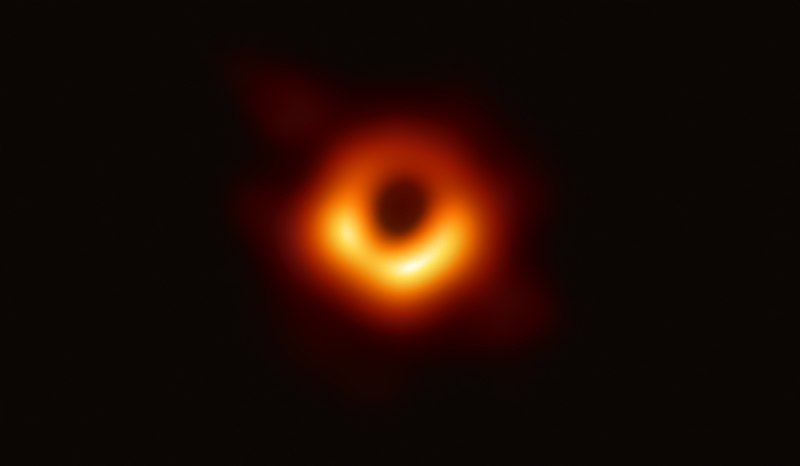
\includegraphics[width=8cm]{Black Hole Image.jpg}
\caption{An Image of a Black Hole, as studied in \textcite{hawking_particle_1993}}
\end{figure}

\section*{Major Heading}
Etiam a mi cursus, vehicula magna id, vestibulum urna. Vivamus pharetra arcu tellus, eu dignissim felis suscipit ut. Phasellus et ligula aliquam, convallis elit quis, ullamcorper purus. Etiam turpis ligula, tincidunt sed tincidunt nec, pellentesque nec est. Fusce non mollis mi. Mauris ut elit tempor, euismod erat nec, lacinia metus. Morbi maximus neque dolor, nec pulvinar dui scelerisque et. Vestibulum efficitur mollis lobortis. In hac habitasse platea dictumst. Vestibulum ut nibh et felis scelerisque mattis a at mauris. Aliquam erat volutpat. Vivamus vel massa egestas, tempor dolor ac, imperdiet ipsum.

Etiam nec malesuada ex. Vestibulum laoreet purus nec metus egestas, sit amet fringilla ipsum laoreet. Pellentesque ornare, neque in convallis maximus, quam mi facilisis felis, sed cursus dui lectus sit amet felis. Proin finibus quis urna ut sollicitudin. Vestibulum congue, ex vitae suscipit efficitur, elit quam ullamcorper est, eget tempus mi velit eget mi. Integer eget nunc eu eros cursus bibendum. Vestibulum ultrices ligula quis nulla porta malesuada. Morbi vel mi vel erat tempor consectetur sed a arcu. Phasellus convallis nibh ut erat posuere, a pharetra ipsum viverra. Praesent scelerisque maximus urna. Nam mattis ac massa in scelerisque. Praesent vulputate feugiat diam id eleifend. Phasellus iaculis ut lectus vestibulum volutpat \autocite{amjad_value_2020}.

\pagebreak

\printbibliography % Be sure to remove access date and months from the .bib file
\end{document}
